%% ELEC 451 - Lab 0 report
%% Layout based on the IEEEtran lab report template (EEET2493 template, modified).
%% Sections: Introduction, Simulation, Experiment, Conclusion.
%%
%% Search for "TODO" in this file for the few places that need your attention.
%% Figures are expected in the images/ folder next to this file.

\documentclass[journal,onecolumn]{IEEEtran}

% *** MATH ***
\usepackage{amsmath}

% *** FIGURES ***
\usepackage{graphicx}
\usepackage{float}
% looks for images in images/ (or report/images/ or the main folder)
\graphicspath{{images/}{report/images/}{./}}
% IEEE-recommended way to get (a), (b), (c) sub-figures with IEEEtran
\usepackage[caption=false,font=footnotesize]{subfig}

% *** PDF, URL AND HYPERLINK PACKAGES ***
\usepackage{hyperref}

% correct bad hyphenation here
\hyphenation{op-tical net-works semi-conduc-tor}

\begin{document}

% paper title
\title{ELEC 451 Power Electronics\\
Lab 0: Introduction to Simulations and Experimental Instruments}

% author names
\author{Student Name 1, 00000000,
        Student Name 2, 00000000,
        Student Name 3, 00000000% <-this % stops a space
}

% The report headers
\markboth{ELEC 451 Power Electronics. Lab Report 0, September 2026}%
{ELEC 451 Power Electronics. Lab Report 0, September 2026}

% make the title area
\maketitle

%% ====================================================================
\section{Introduction}
\label{sec:intro}

\IEEEPARstart{T}{his} is Lab~0 of ELEC~451. Its principal focus is on the
basics of PSIM, the proper use and calibration of the measurement probes used
in the lab (passive, differential and current probes), and performing
mathematics such as the Fast Fourier Transform (FFT) in both PSIM and on the
oscilloscope.

Successful completion and understanding of the lab allows the team to
progress through the rest of the labs while spending minimal time on learning
the basics of the equipment.

The overarching scientific objective of this lab, in addition to the
practical skills, is to demonstrate how simulation and real-world results
differ or overlap.

This report is organized as follows. Section~\ref{sec:sim} presents the PSIM
simulations: circuit setup, transient and steady-state waveforms, the effect
of the time step, mean-value measurements and the FFT.
Section~\ref{sec:exp} describes the experimental work with the oscilloscope:
probe calibration, time-domain measurements and the FFT.
Section~\ref{sec:conc} concludes the report.

%% ====================================================================
\section{Simulation}
\label{sec:sim}

\subsection{Circuit Setup (Activity 1)}

The circuit in Fig.~\ref{fig:schematic} was built in PSIM. A 10~kHz
square-wave voltage source feeds a 1~mH inductor in series, followed by a
$10~\mu\mathrm{F}$ capacitor in parallel with a $20~\Omega$ resistor. The
source voltage $v_i$, the output voltage $v_o$ and the inductor current $i_L$
are measured with probes placed according to the polarity shown.

\begin{figure}[H]
\centering
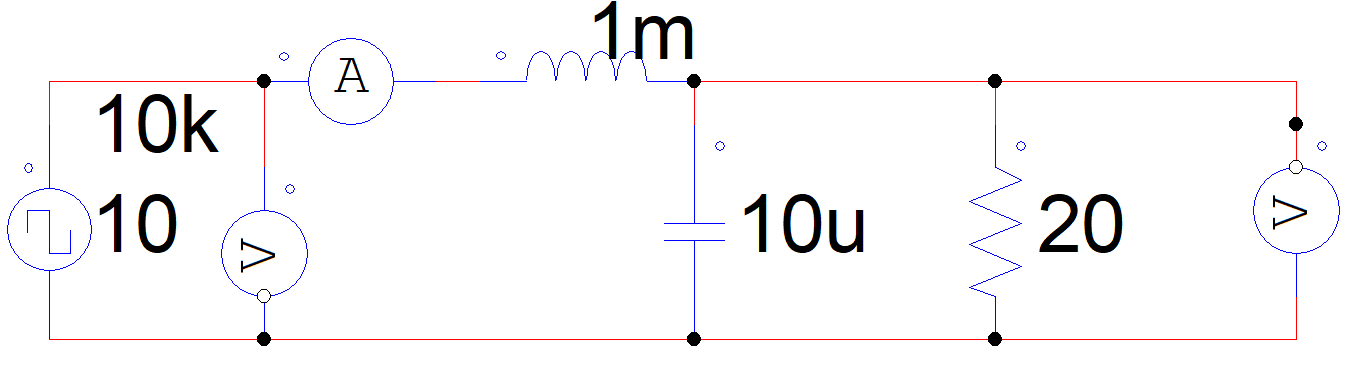
\includegraphics[width=\textwidth]{sim_schematic.png}
\caption{PSIM schematic of the circuit: square-wave source (10~kHz), 1~mH
inductor, $10~\mu\mathrm{F}$ capacitor and $20~\Omega$ resistor, with voltage
probes $v_i$ and $v_o$ and inductor current probe $i_L$.}
\label{fig:schematic}
\end{figure}

\subsection{Waveform Captures (Activities 2 and 3)}

Fig.~\ref{fig:a2} shows $v_i$, $v_o$ and $i_L$ over the first 5.5~ms as first
captured. The square-wave source correctly swings between 0~V and 10~V, as
specified in Table~\ref{tab:params}; $v_o$ overshoots to about 7.3~V before
settling to a steady-state ripple around 5~V.

The Simulation Control tool was then added, with a time step of
$1~\mu\mathrm{s}$ and a total time of 2~ms, so that the complete transient of
the signals is visible (Fig.~\ref{fig:a3}); the signals reach steady state
after roughly 1~ms. Fig.~\ref{fig:a3zoom} zooms in to five cycles of the
steady-state waveforms.

% TODO: add the component-value table referenced above if you don't already
% have one (Table~\ref{tab:params}), or replace the cross-reference with the
% values directly.

\begin{figure}[H]
\centering
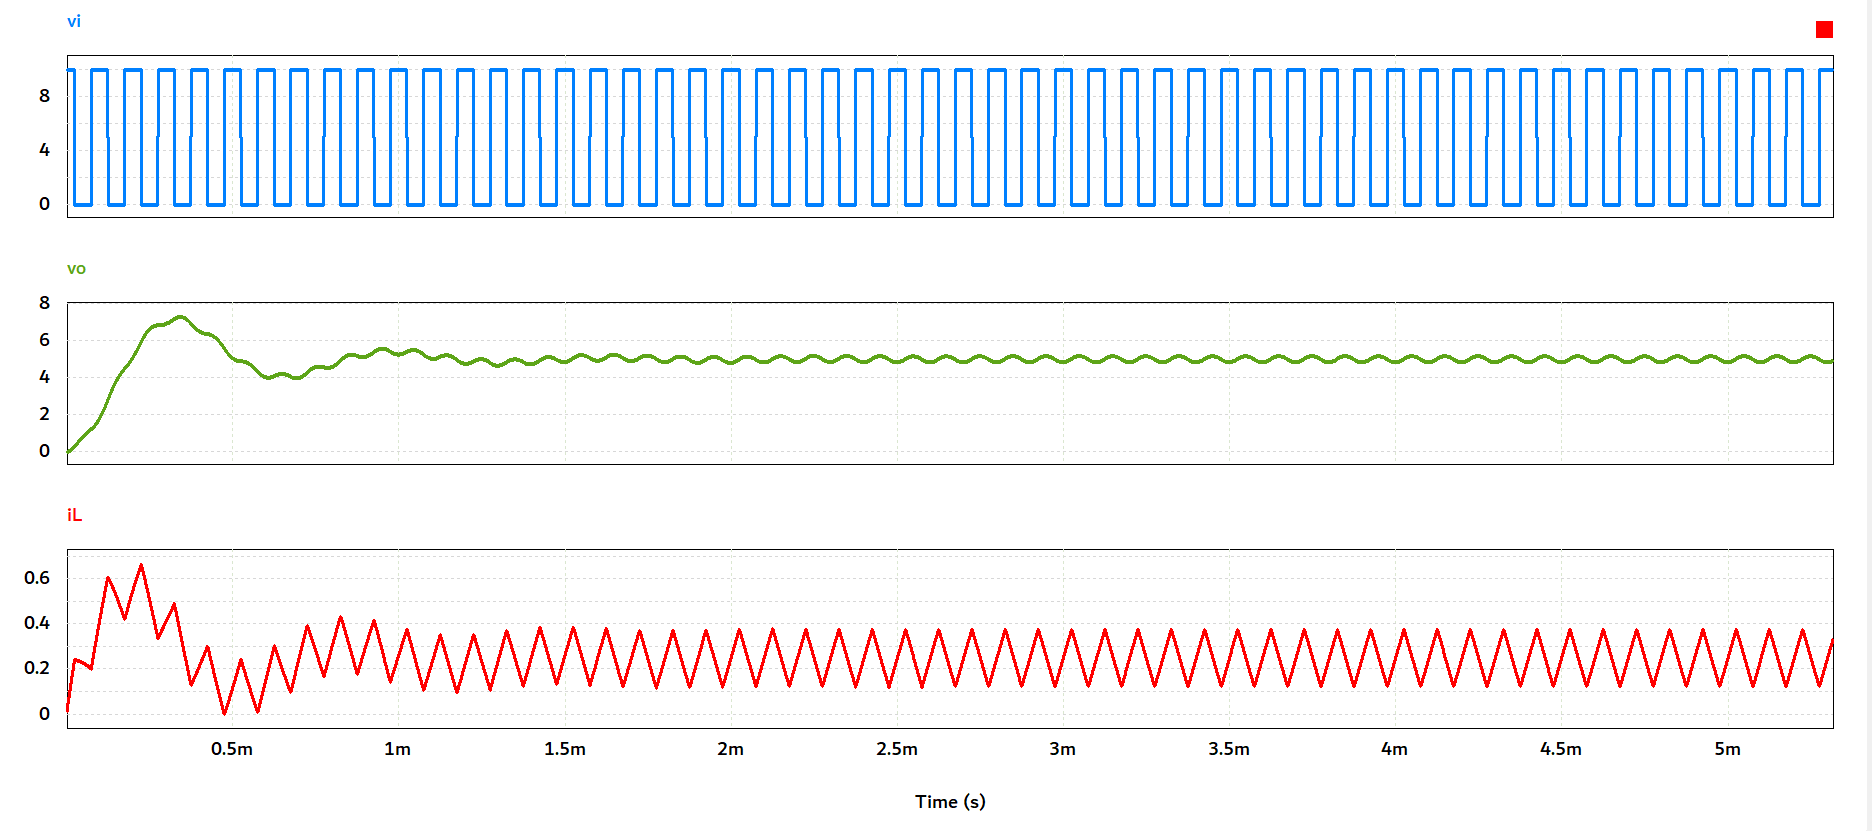
\includegraphics[width=\textwidth]{sim_a2_combined.png}
\caption{Simulated waveforms $v_i$, $v_o$ and $i_L$ (top to bottom) as first
captured.}
\label{fig:a2}
\end{figure}

\begin{figure}[H]
\centering
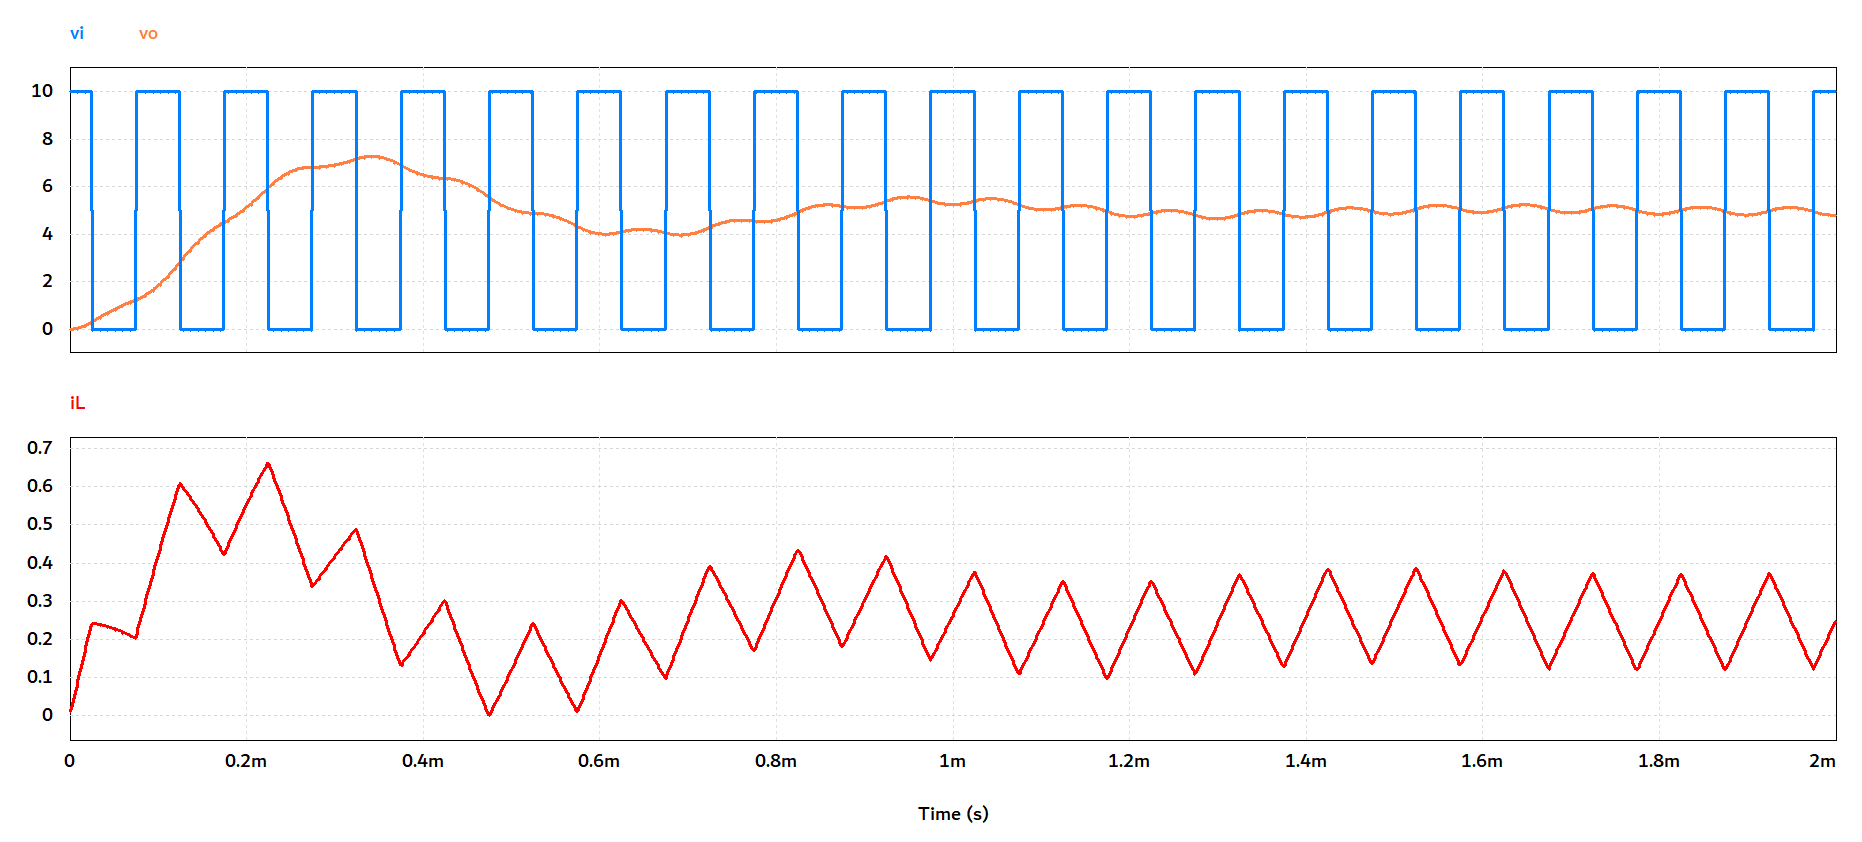
\includegraphics[width=\textwidth]{sim_a3_combined.png}
\caption{Transient and steady-state waveforms with a $1~\mu\mathrm{s}$ time
step and a total time of 2~ms: $v_i$ and $v_o$ overlaid (top), $i_L$
(bottom).}
\label{fig:a3}
\end{figure}

\begin{figure}[H]
\centering
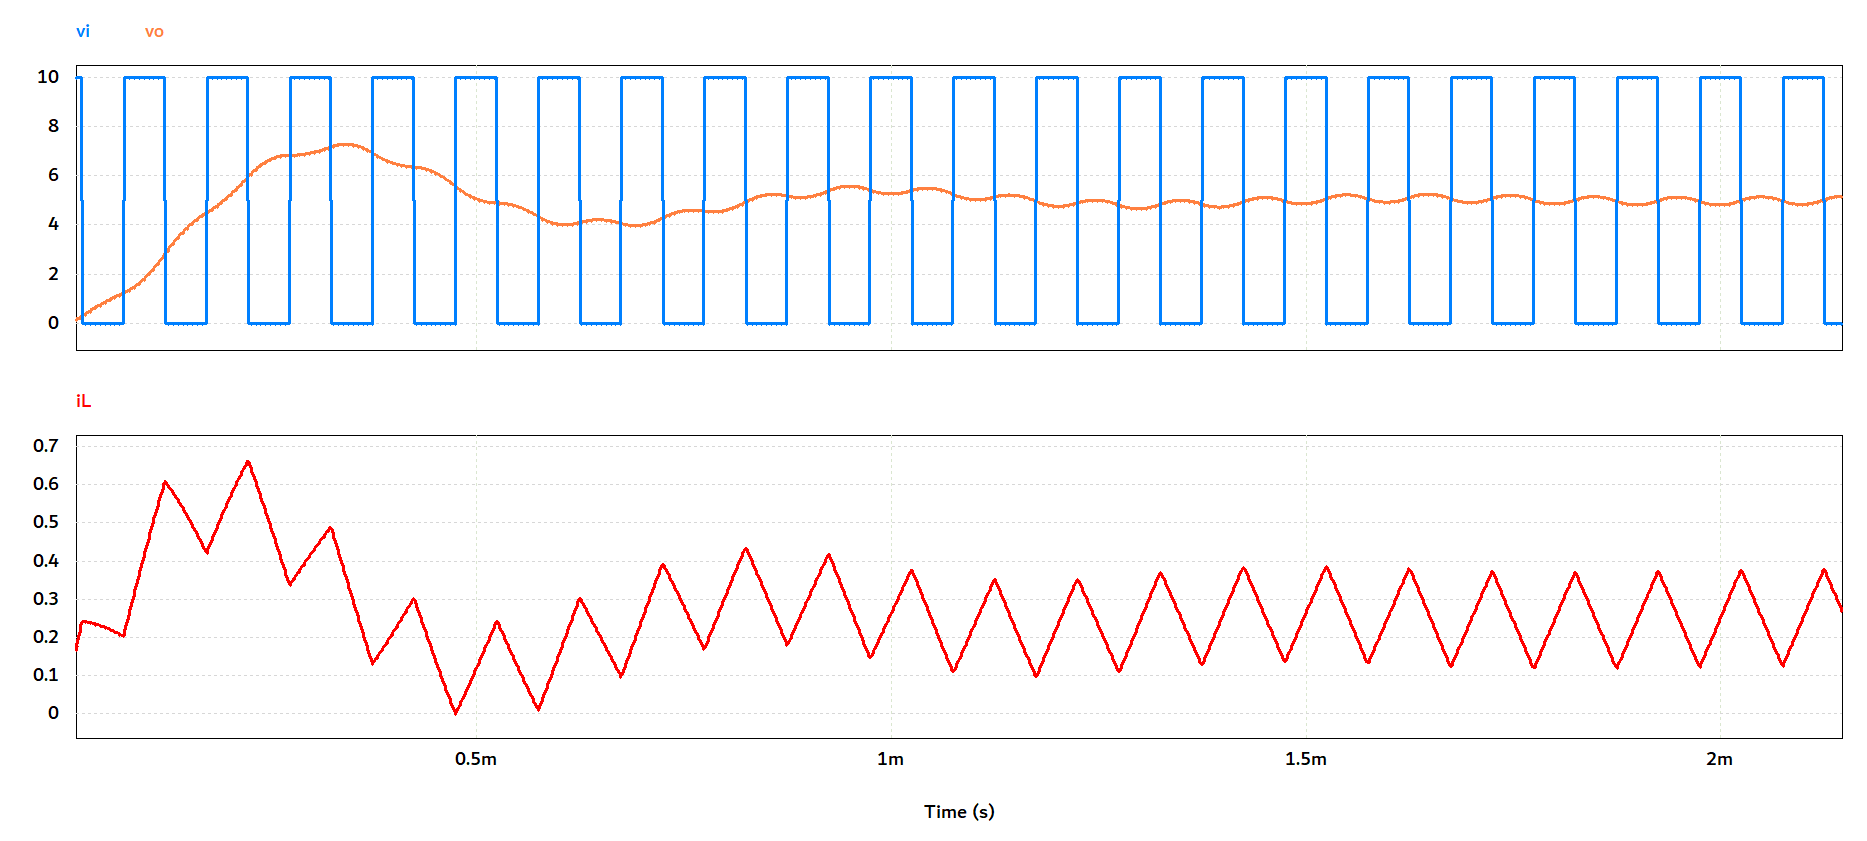
\includegraphics[width=\textwidth]{sim_a3zoom_combined.png}
\caption{Five cycles of the steady-state waveforms: $v_i$ and $v_o$ overlaid
(top), $i_L$ (bottom).}
\label{fig:a3zoom}
\end{figure}

\subsection{Time Step (Activity 4)}

The waveforms were captured for a large time step ($1\times10^{-5}$~s,
Fig.~\ref{fig:a4large}), a reasonable time step
% TODO: confirm this value -- it was not shown on the capture.
($1~\mu\mathrm{s}$, Fig.~\ref{fig:a4mid}) and a very small time step
% TODO: confirm this value -- it was not shown on the capture.
($1\times10^{-7}$~s, Fig.~\ref{fig:a4small}).
% TODO: at the 2 ms / 20-cycle scale shown here, the three captures look
% nearly identical -- the distortion from the large step is not clearly
% visible. Consider zooming to 5 steady-state cycles (as the lab asks) so the
% difference between the three step sizes is visible, and adjust the sentence
% below to match what you actually see.
Even at this scale, the waveforms remain clean, since $20~\Omega$ load
strongly damps the ringing regardless of step size; a closer, few-cycle zoom
would be needed to see any edge distortion at the largest step.

The more time steps taken, the longer the software takes to process the
simulation. A smaller time step also helps to avoid aliasing and clipping of
the signal.

\begin{figure}[H]
\centering
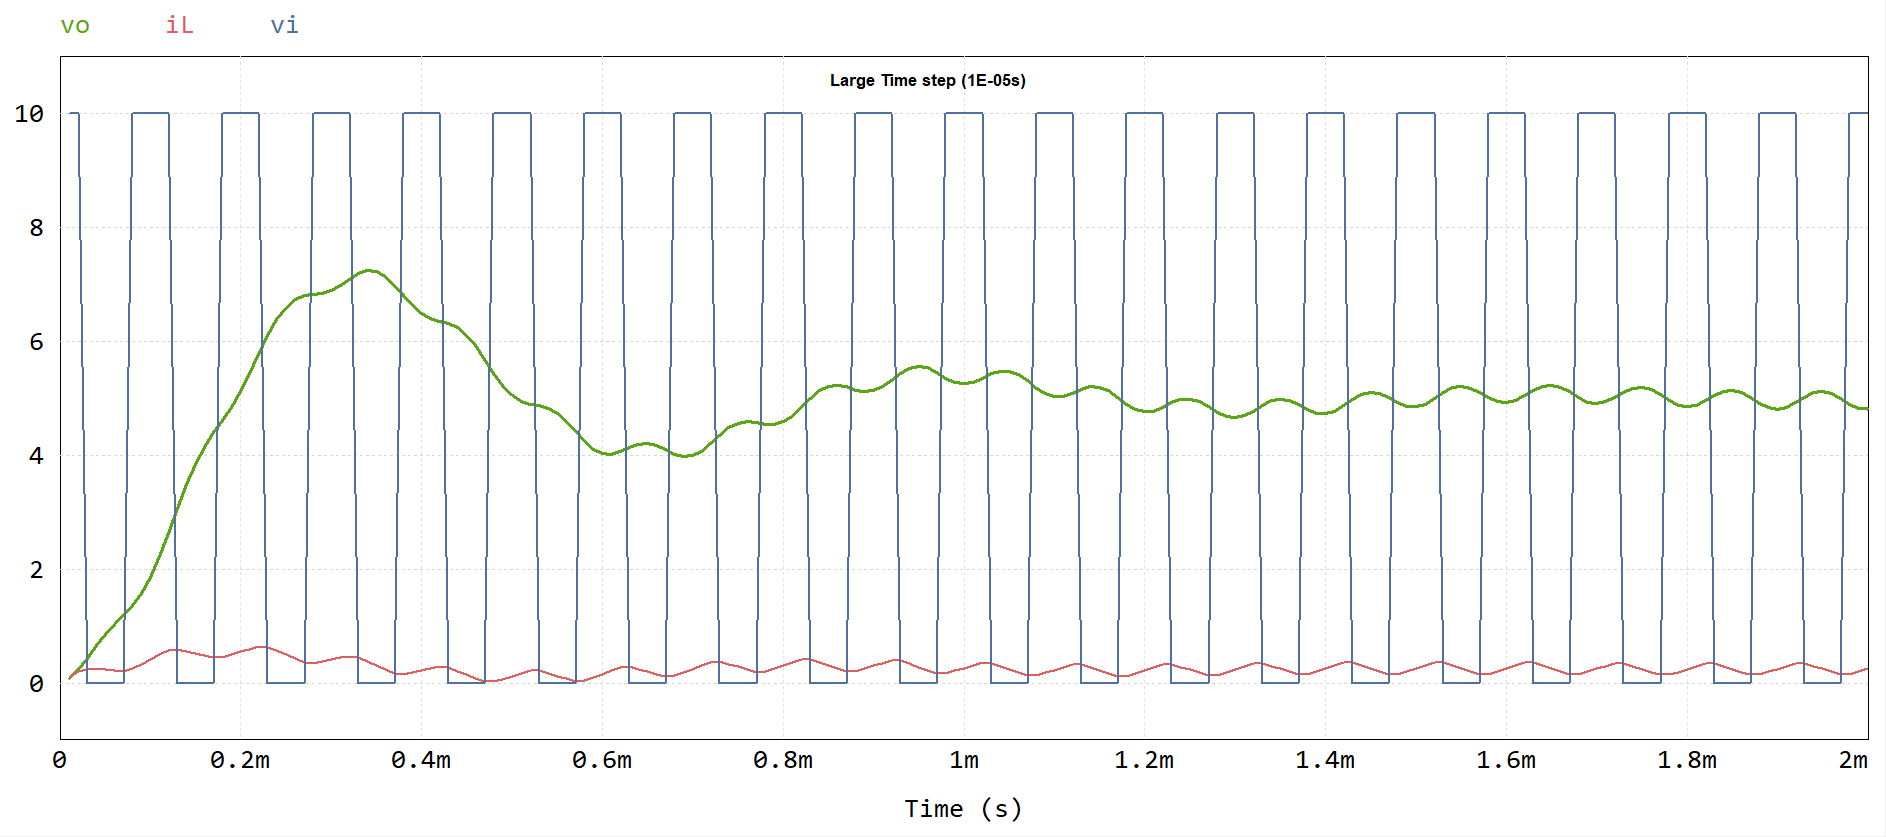
\includegraphics[width=\textwidth]{sim_a4_large_combined.png}
\caption{Waveforms with a large time step ($1\times10^{-5}$~s): $v_i$, $v_o$
and $i_L$ overlaid.}
\label{fig:a4large}
\end{figure}

\begin{figure}[H]
\centering
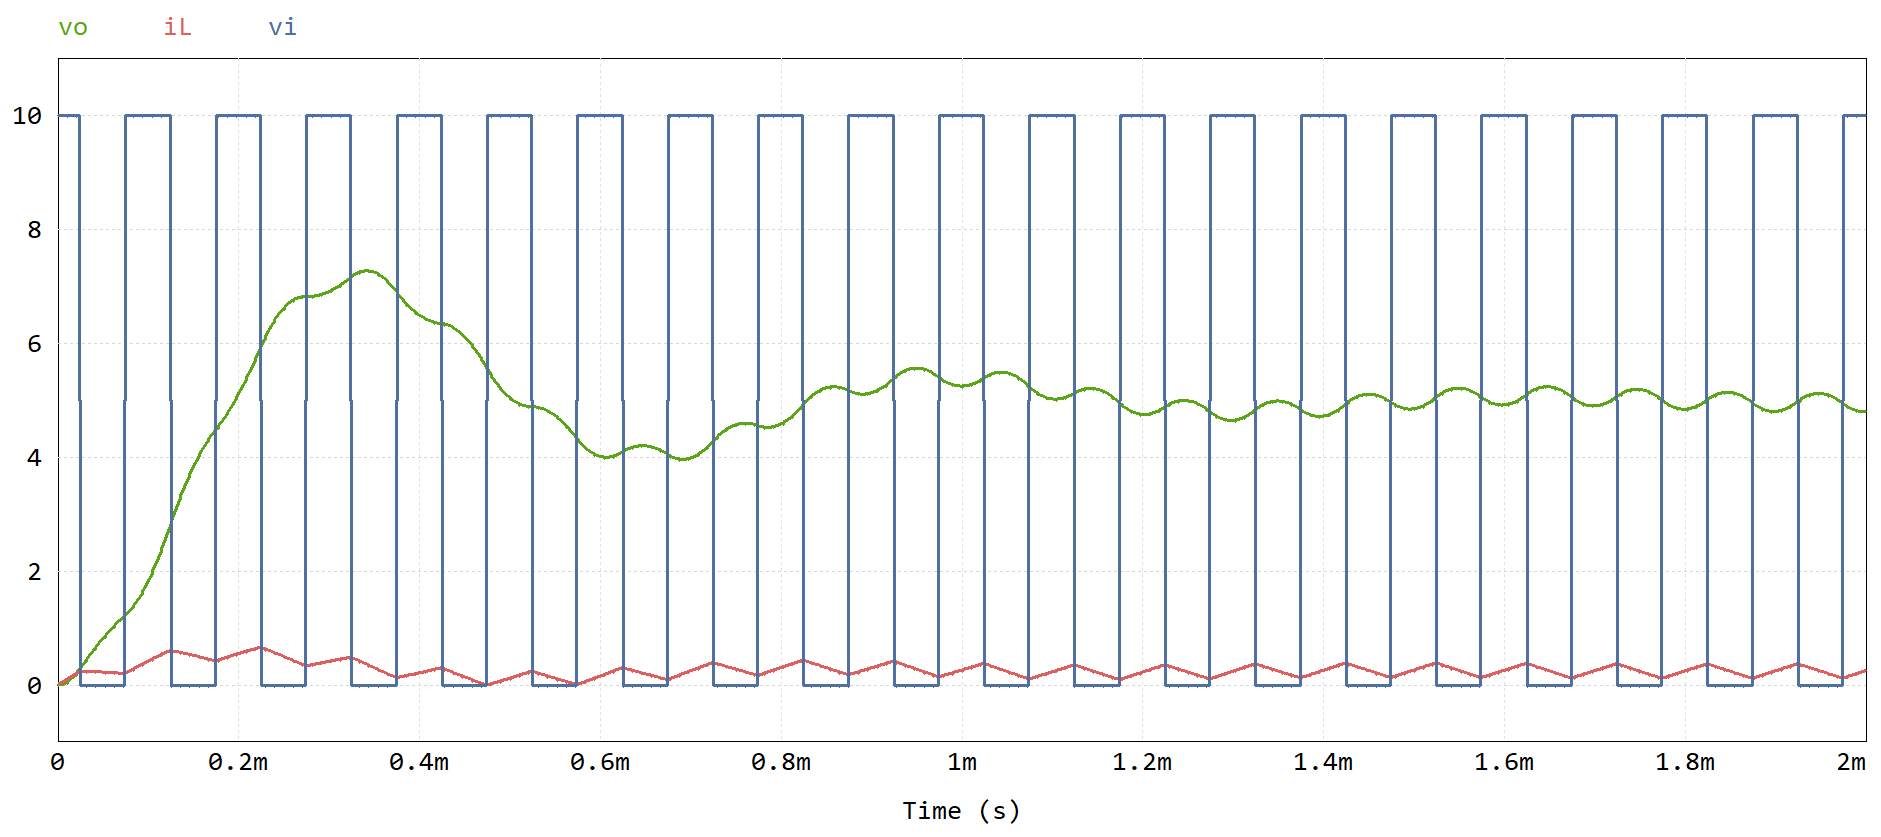
\includegraphics[width=\textwidth]{sim_a4_mid_combined.png}
\caption{Waveforms with a reasonable time step ($1~\mu\mathrm{s}$): $v_i$,
$v_o$ and $i_L$ overlaid.}
\label{fig:a4mid}
\end{figure}

\begin{figure}[H]
\centering
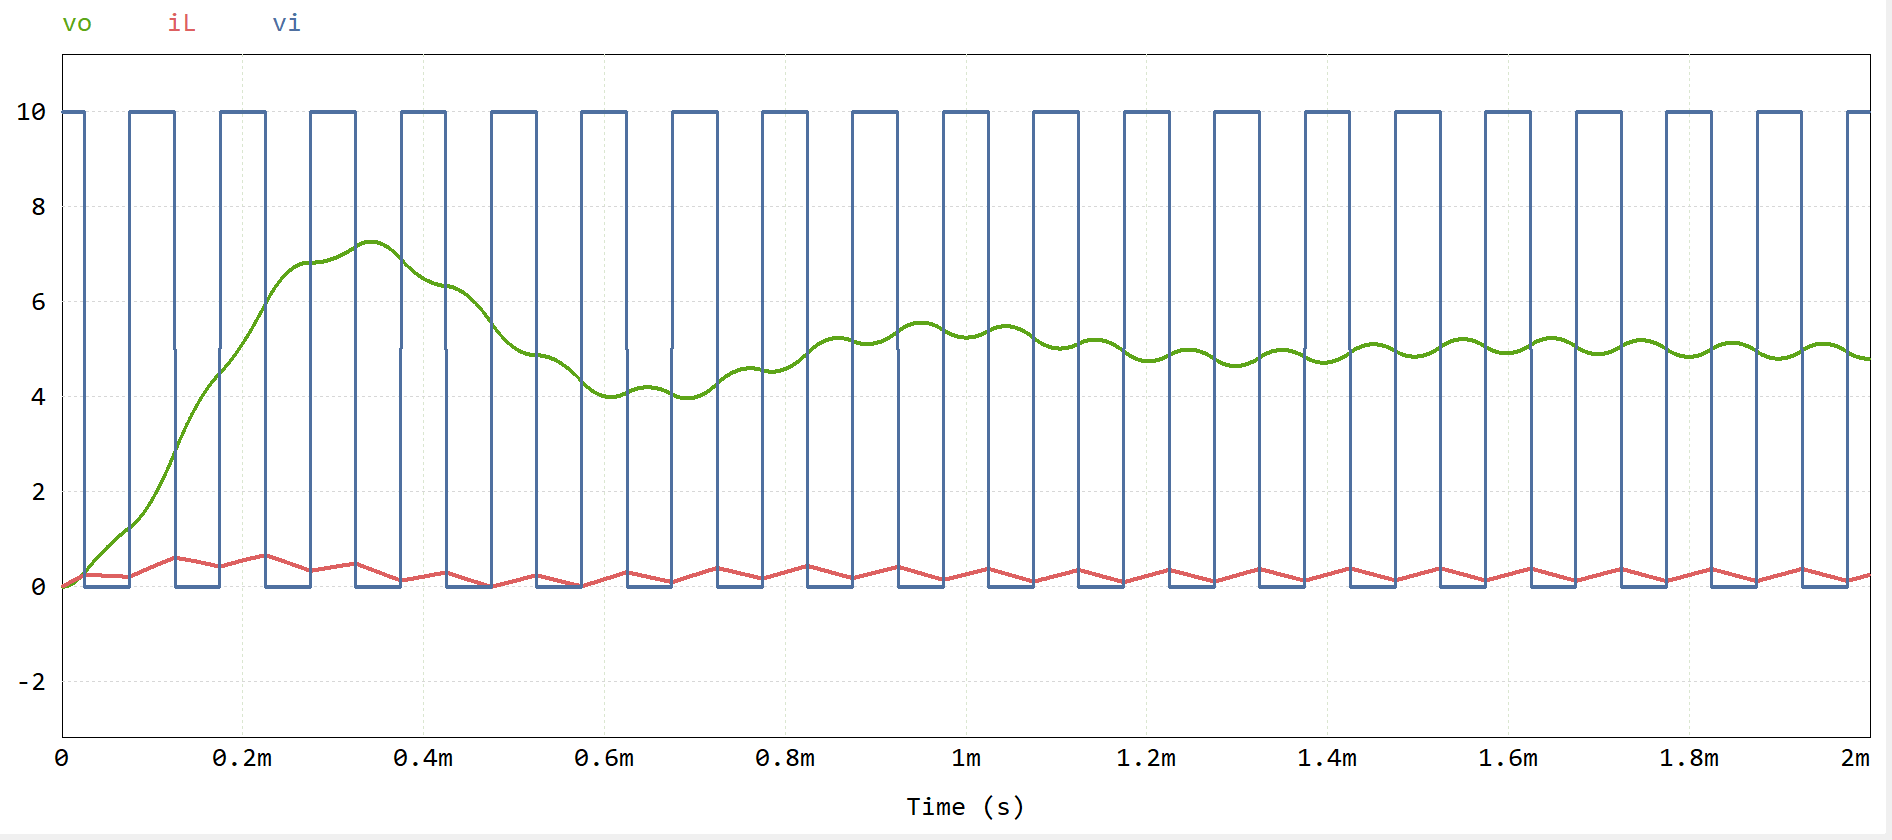
\includegraphics[width=\textwidth]{sim_a4_small_combined.png}
\caption{Waveforms with a very small time step ($1\times10^{-7}$~s): $v_i$,
$v_o$ and $i_L$ overlaid.}
\label{fig:a4small}
\end{figure}

\subsection{Measurements (Activity 5)}

The mean value of $v_o$ and $i_L$ was measured with the Measure cursor tool
over 10 complete steady-state cycles (1.00~ms). The results are listed in
Table~\ref{tab:means}.
% TODO: this table now has only the 10-cycle row, with vi still missing.
% The 2.5-cycle and 50-cycle rows, and the vi mean, from the previous
% (incorrect) simulation have been removed since they have not been
% re-measured. If you still have those, or the vi value, send them and I'll
% add the rows back and restore the comparison discussion.

\begin{table}[H]
\renewcommand{\arraystretch}{1.2}
\caption{Mean values over 10 steady-state cycles}
\label{tab:means}
\centering
\begin{tabular}{lcc}
\hline
Time span & $v_o$ (V) & $i_L$ (A)\\
\hline
10 cycles  & 5.007 & 0.2495\\
\hline
\end{tabular}
\end{table}

Fig.~\ref{fig:a5meas} shows the corresponding Measure-tool captures for $v_o$
and $i_L$.

\begin{figure}[H]
\centering
\subfloat[Output voltage $v_o$.]{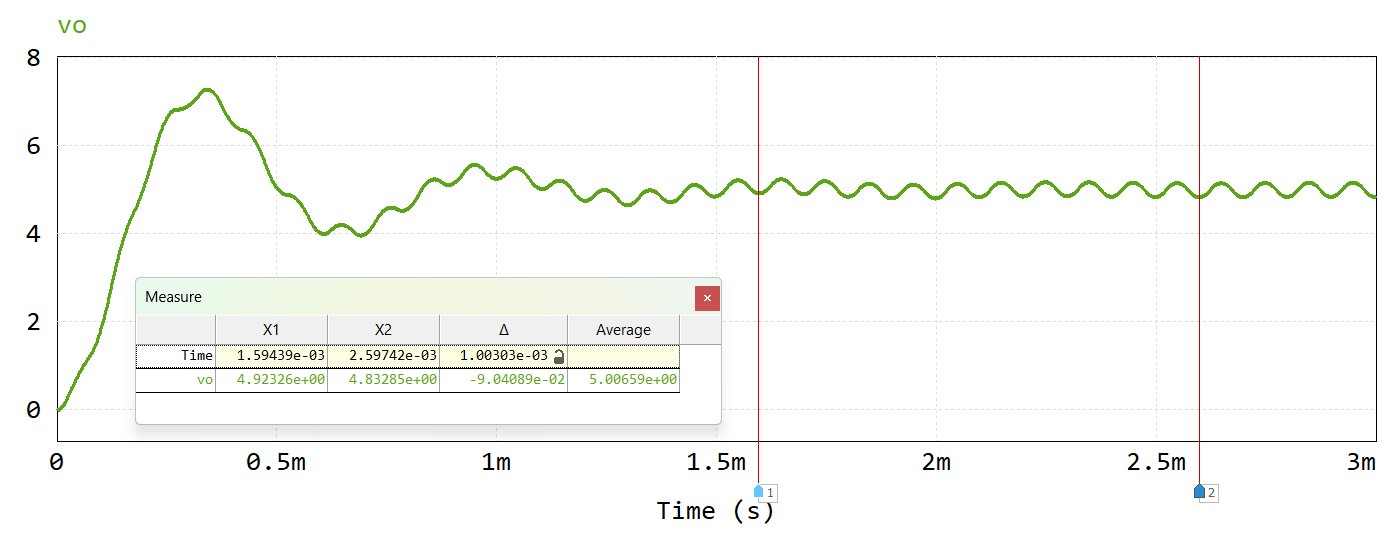
\includegraphics[width=0.48\textwidth]{sim_a5_vo_mean.png}}\hfill
\subfloat[Inductor current $i_L$.]{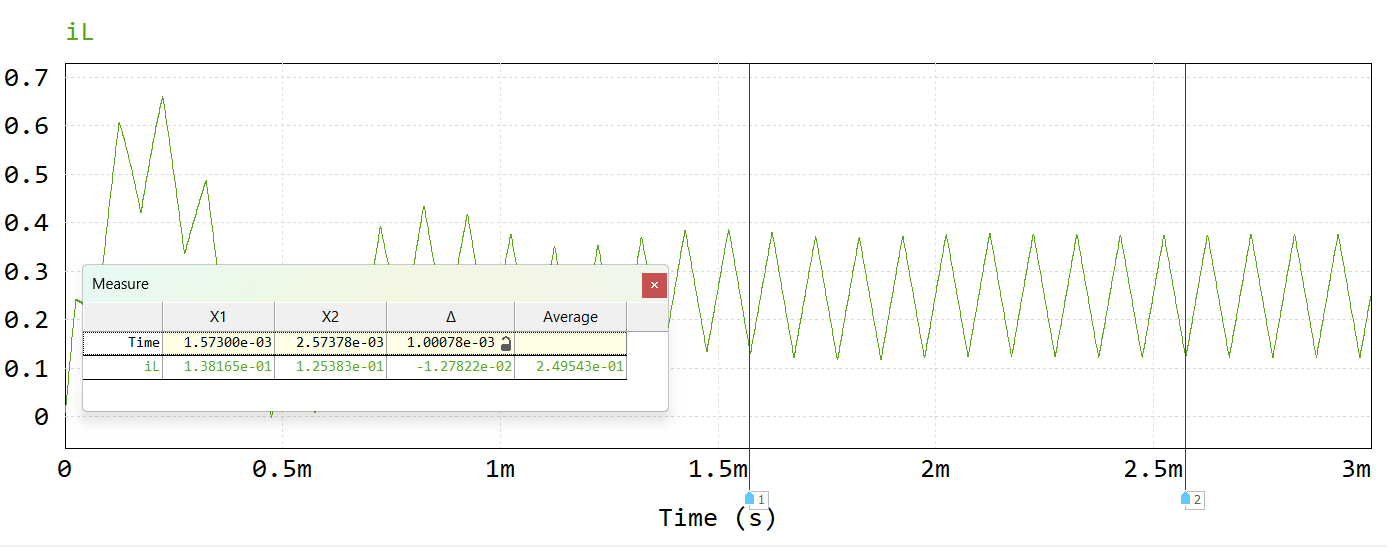
\includegraphics[width=0.48\textwidth]{sim_a5_il_mean.png}}
\caption{Mean-value measurements over 10 steady-state cycles (1.00~ms).}
\label{fig:a5meas}
\end{figure}

% TODO: the peak inductor-current capture from Activity 5c (Mark Data Point)
% is not part of this batch of images -- if you have re-run it, send it over
% and I'll add it back here with the new peak value and timestamp.

\subsection{FFT (Activity 6)}

The triangular-wave voltage source (10~kHz, 1~V peak-to-peak, 2~V DC offset)
was simulated and its FFT computed with Analysis/Perform FFT
(Fig.~\ref{fig:a6default}); the fundamental appears clearly at 10~kHz.
% TODO: confirm the total simulation time used for this default capture.

The total simulation time was then reduced to below 10 cycles
(Fig.~\ref{fig:a6short}(a)); the resulting FFT (Fig.~\ref{fig:a6short}(b))
shows a wider, less well-defined peak at 10~kHz because of the coarser
frequency resolution. With the total time increased instead
(Fig.~\ref{fig:a6long}), the fundamental at 10.0~kHz and the third harmonic at
30.1~kHz are both sharply resolved.
% TODO: the step-size sub-part of Activity 6 (step 10x and 100x smaller,
% Fig. 10 in the previous version) is not part of this batch either. Send
% those over if you have re-run them and I'll add that comparison back.

\begin{figure}[H]
\centering
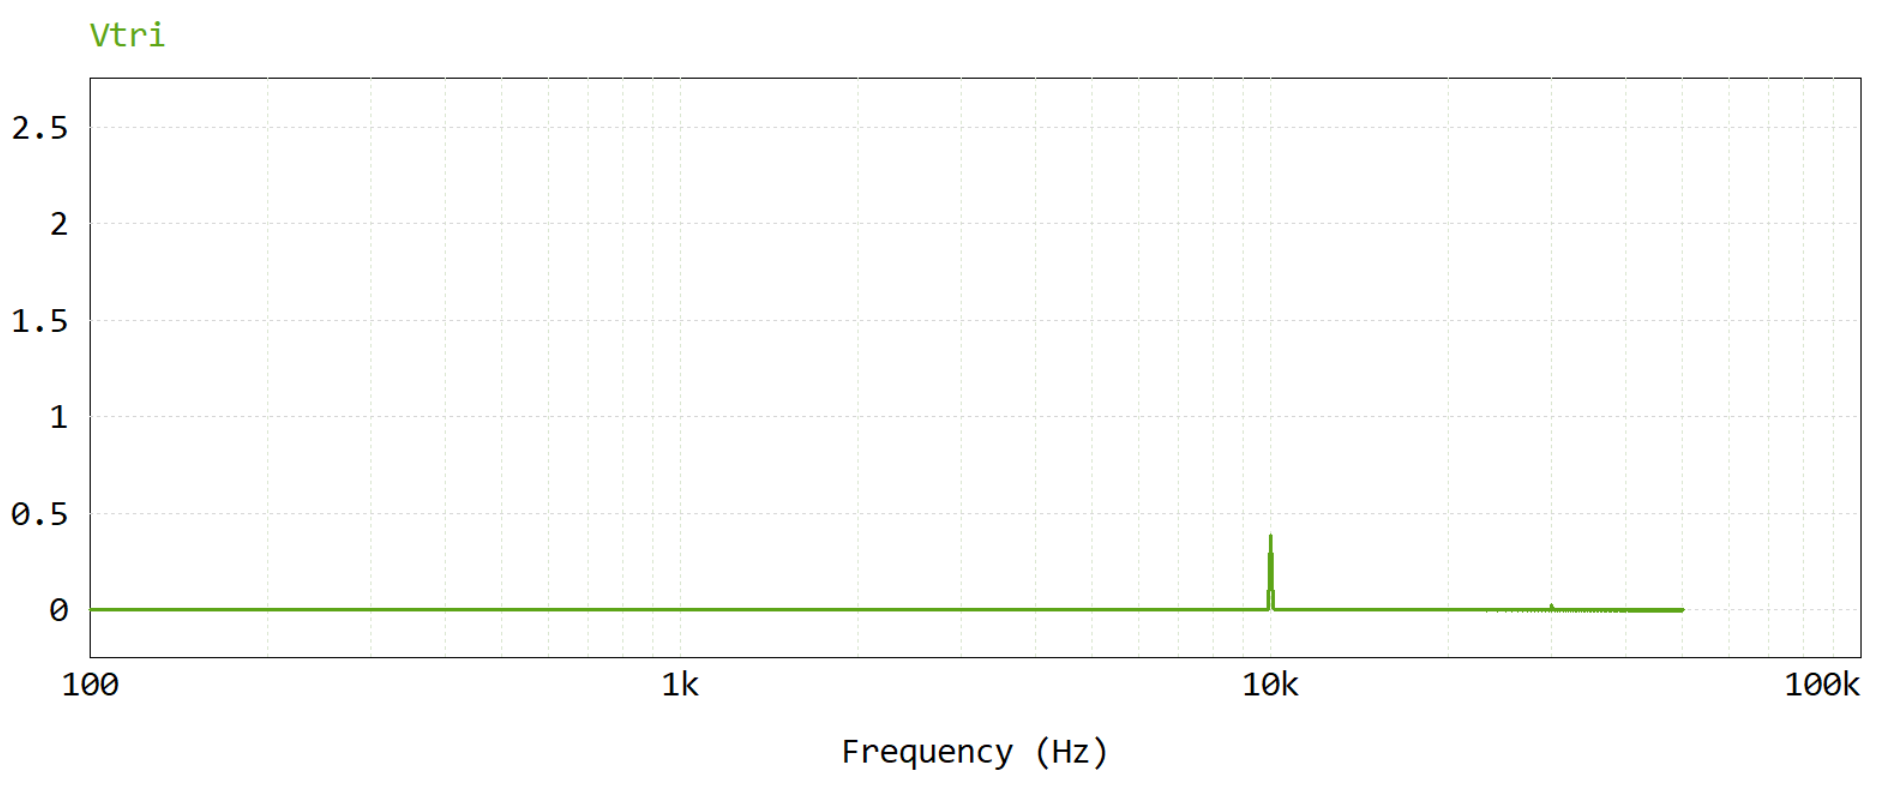
\includegraphics[width=\textwidth]{sim_a6_fft_default.png}
\caption{FFT of the triangular-wave voltage, full span.}
\label{fig:a6default}
\end{figure}

\begin{figure}[H]
\centering
\subfloat[Time-domain waveform.]{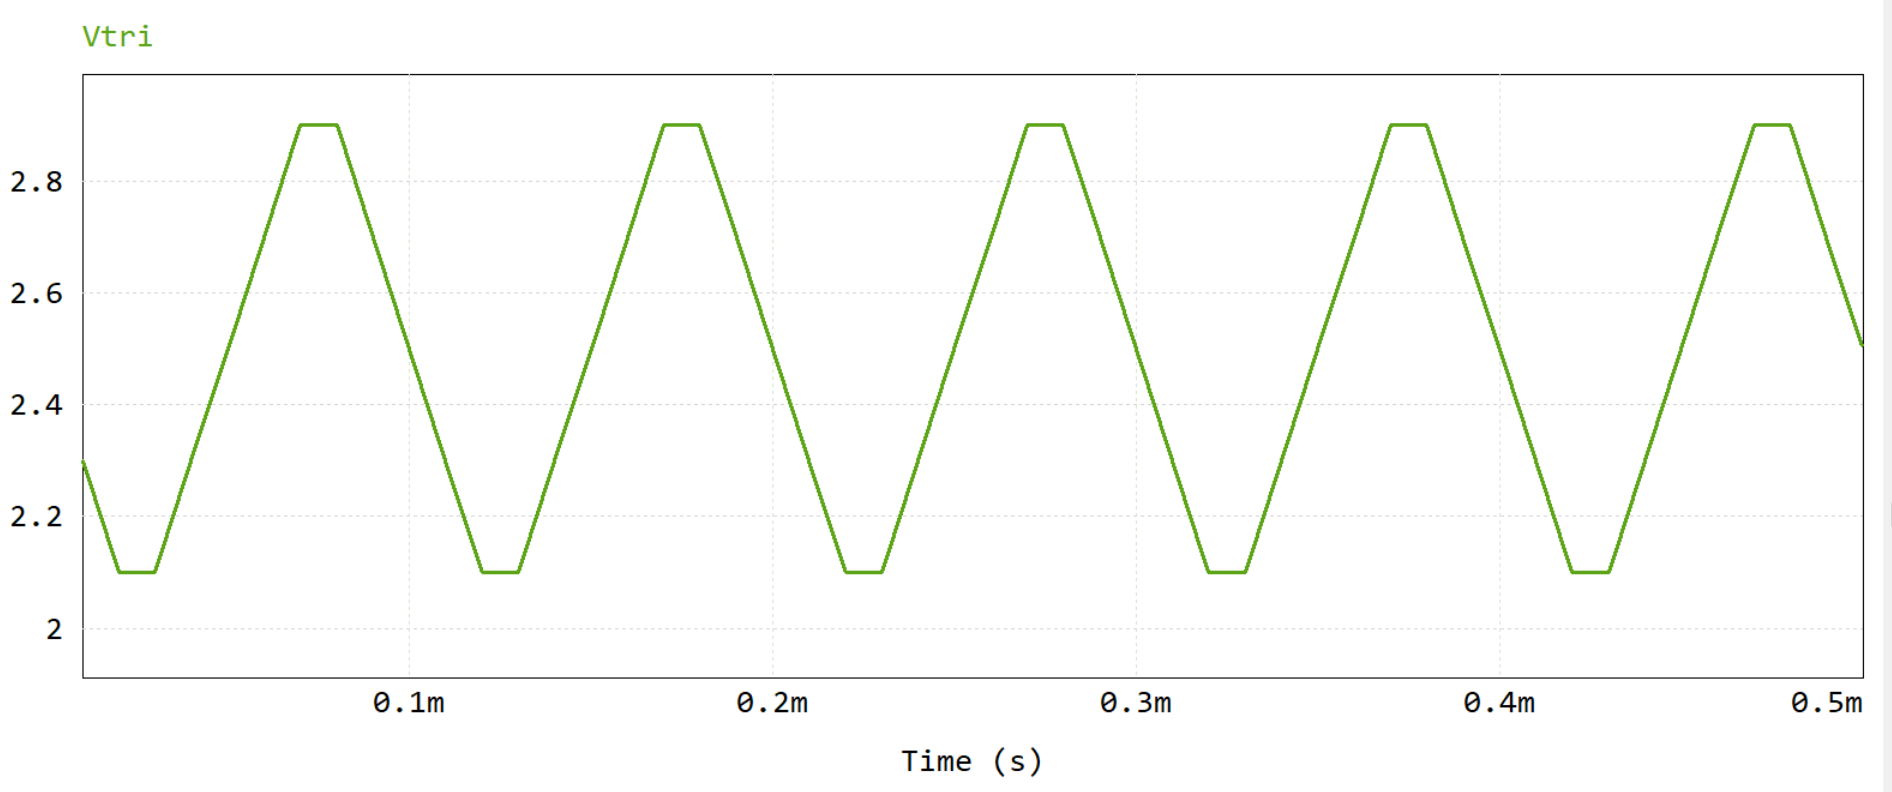
\includegraphics[width=0.48\textwidth]{sim_a6_shorttime_wave.png}}\hfill
\subfloat[Corresponding FFT.]{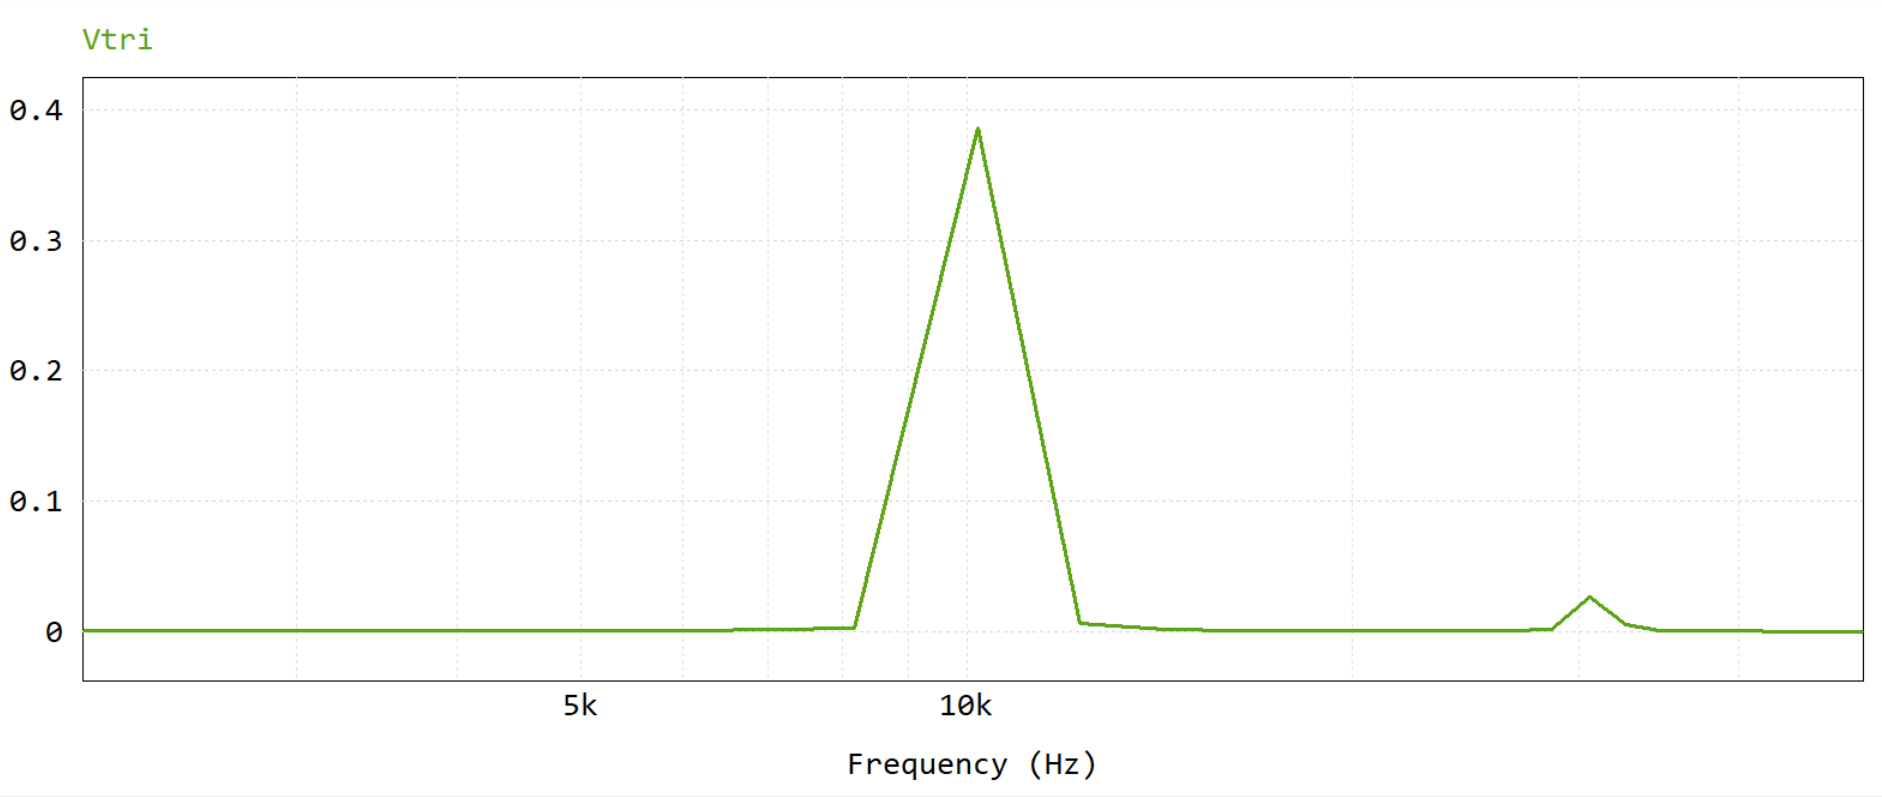
\includegraphics[width=0.48\textwidth]{sim_a6_fft_shorttime.png}}
\caption{Triangular-wave voltage with the total simulation time reduced to
below 10 cycles.}
\label{fig:a6short}
\end{figure}

\begin{figure}[H]
\centering
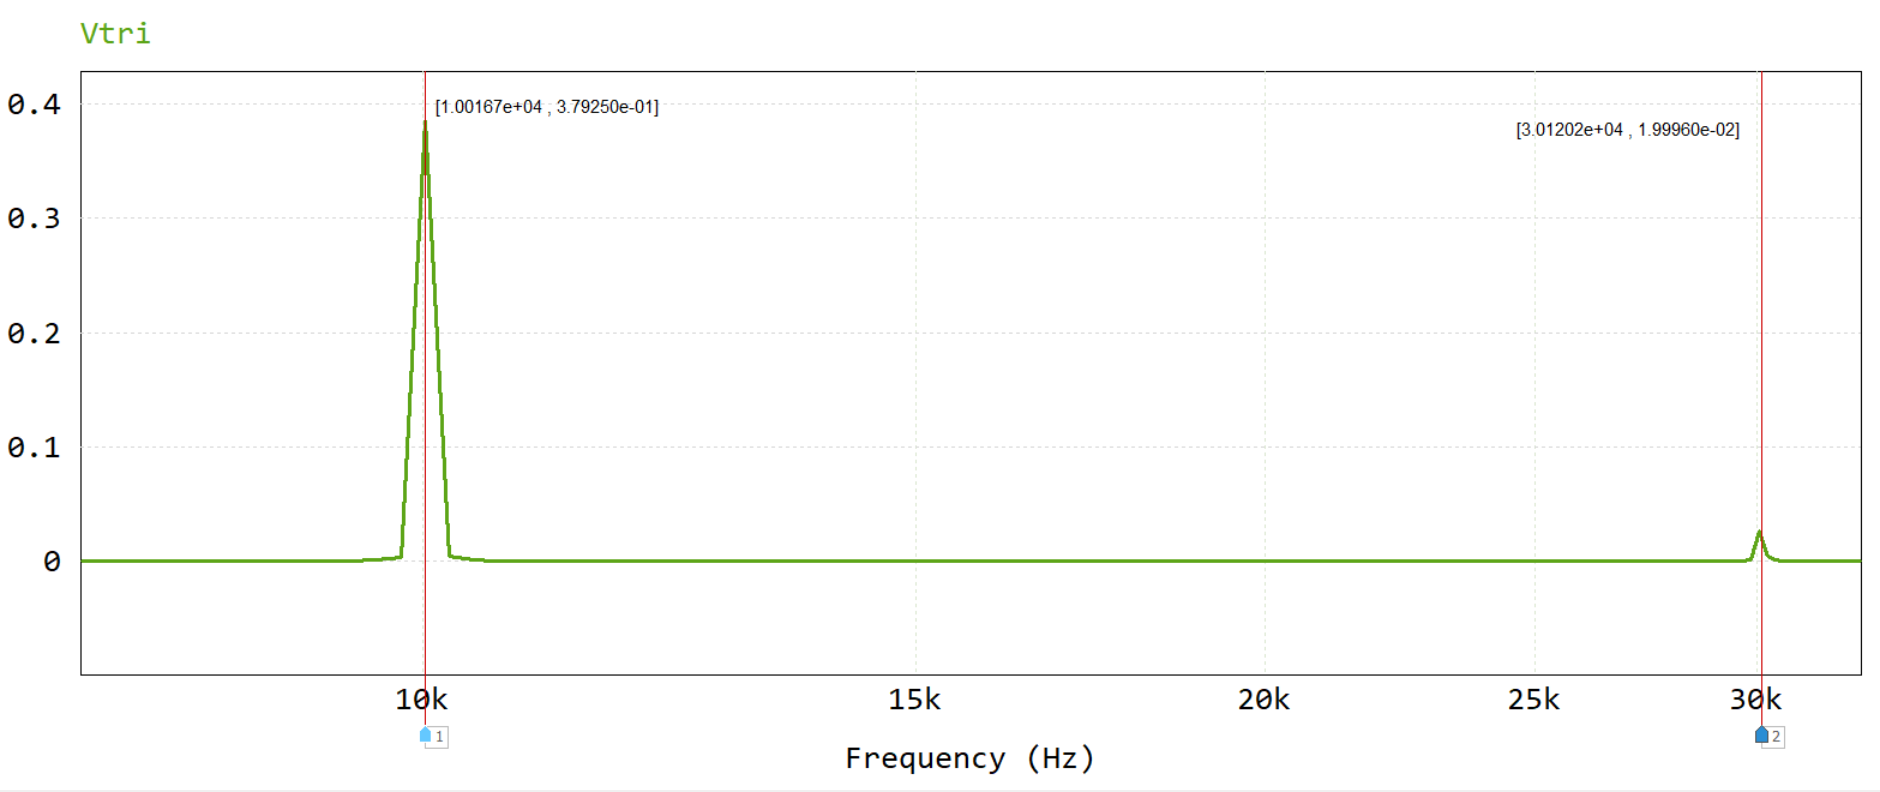
\includegraphics[width=\textwidth]{sim_a6_fft_longtime.png}
\caption{FFT of the triangular-wave voltage with the total simulation time
increased to more than 10 cycles. Cursors mark the fundamental
(10.02~kHz, 0.379) and the third harmonic (30.12~kHz, 0.020).}
\label{fig:a6long}
\end{figure}

A longer total simulation time gives finer frequency resolution and a
sharper, more legible FFT, while a short total time smears the peaks and
makes the harmonics harder to distinguish. This reinforces the same
Shannon--Nyquist trade-off encountered when varying the time step: enough
samples, over a long enough window, are needed to resolve the spectrum
clearly.

%% ====================================================================
\section{Experiment}
\label{sec:exp}

\subsection{Probe Calibration (Activity 1)}

Before taking measurements, the probes were configured and calibrated against
the calibration signal of the oscilloscope (a 1~kHz square wave)
(Fig.~\ref{fig:cal}).

% TODO: no notes/capture for the current probe -- add a sentence if you did it.
\begin{figure}[H]
\centering
\subfloat[Passive probe: clean test waveform.]{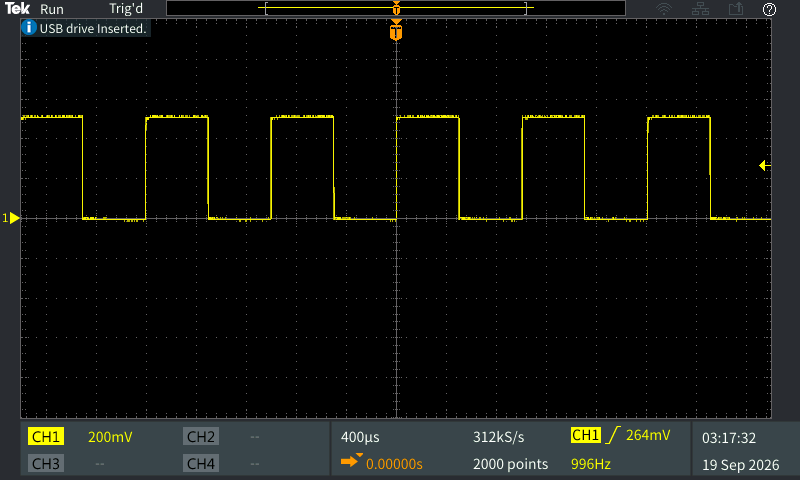
\includegraphics[width=0.48\textwidth]{exp_cal_passive.png}}\hfill
\subfloat[Differential probe.]{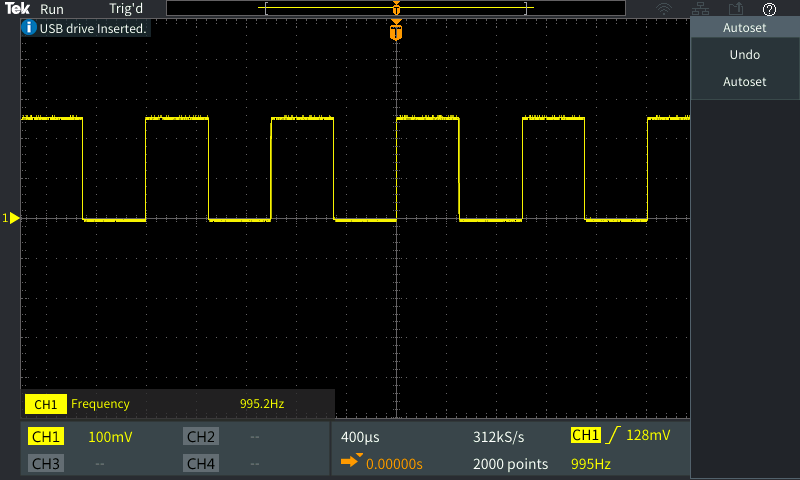
\includegraphics[width=0.48\textwidth]{exp_cal_differential.png}}
\caption{Oscilloscope captures of the calibration signal.}
\label{fig:cal}
\end{figure}

\subsection{Time-Domain Captures and Measurements (Activity 2)}

A triangular wave (10~kHz, 500~mV amplitude, 2~V DC offset) from the function
generator was displayed on the oscilloscope (Fig.~\ref{fig:exp_a2}(a)). The
frequency and mean value measured by the scope (10.00~kHz and 1.995~V) match
the generator settings, and the peak-to-peak amplitude read 560~mV for the
500~mV set on the generator.

When the amplitude was reduced to 10~mV, the details inside the signal became
invisible because of noise. After changing the channel from DC to AC coupling
and applying a high-frequency filter, the triangular shape could be recovered
(Fig.~\ref{fig:exp_a2}(b)): the ripple came into view and, although the signal
was still noisy, it could be analyzed and understood. The automatic
measurements were nevertheless still affected by the noise, with 15.6~mV
peak-to-peak and 17.72~kHz reported for a 10~mV, 10~kHz signal.

% TODO: check the wording above about the 560 mV reading against your own
% conclusion for "Are the values measured by the scope accurate?".
\begin{figure}[H]
\centering
\subfloat[500~mV amplitude, 2~V offset.]{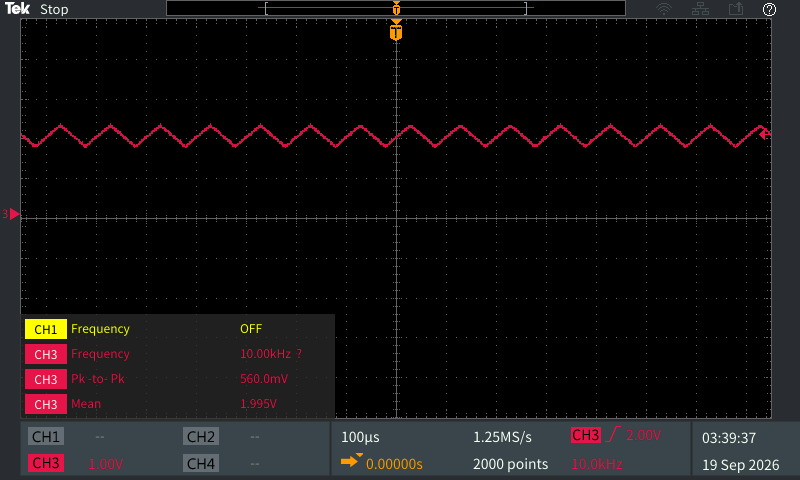
\includegraphics[width=0.48\textwidth]{exp_a2_500mV.png}}\hfill
\subfloat[10~mV amplitude, 2~V offset, AC coupling.]{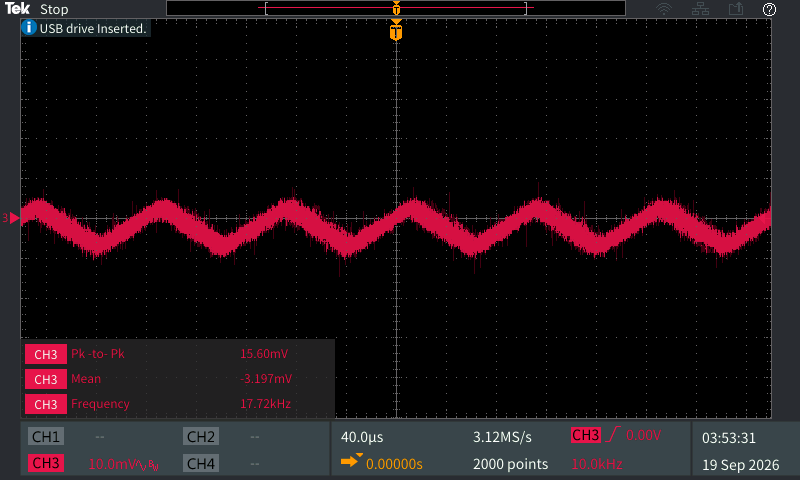
\includegraphics[width=0.48\textwidth]{exp_a2_10mV_ac.png}}
\caption{Oscilloscope captures of the 10~kHz triangular wave.}
\label{fig:exp_a2}
\end{figure}

\subsection{Frequency-Domain Captures and Measurements (Activity 3)}

The team expected the FFT of the 10~kHz triangular wave to show a fundamental
at 10~kHz and further components at integer multiples of it. The captured
spectrum (Fig.~\ref{fig:exp_a3}(a)) shows the fundamental at 10.0~kHz and the
next component at 30.1~kHz.
% TODO: this last sentence replaces the "..." bullet in your notes -- edit as needed.

After changing the signal to 20~kHz, the location of the main spectral line
changed, as expected (Fig.~\ref{fig:exp_a3}(b)). As expected, the pattern of
the harmonics also changed completely when the signal was changed from a
triangular wave to a sine wave (Fig.~\ref{fig:exp_a3}(c)).
% TODO: in panels (b) and (c) the two spectra look almost identical in the
% displayed span. Consider widening the FFT span so the higher triangle
% harmonics are visible, or comment on what is visible.

\begin{figure}[H]
\centering
\subfloat[10~kHz triangular wave.]{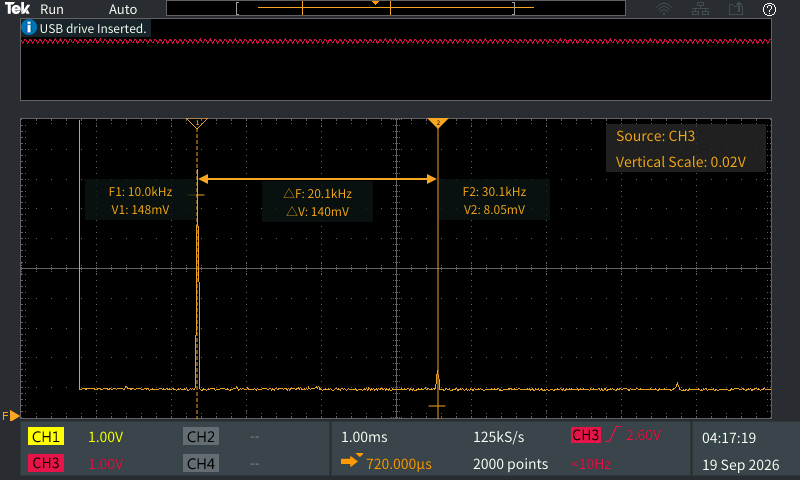
\includegraphics[width=0.48\textwidth]{exp_a3_tri_10kHz.png}}\hfill
\subfloat[20~kHz triangular wave.]{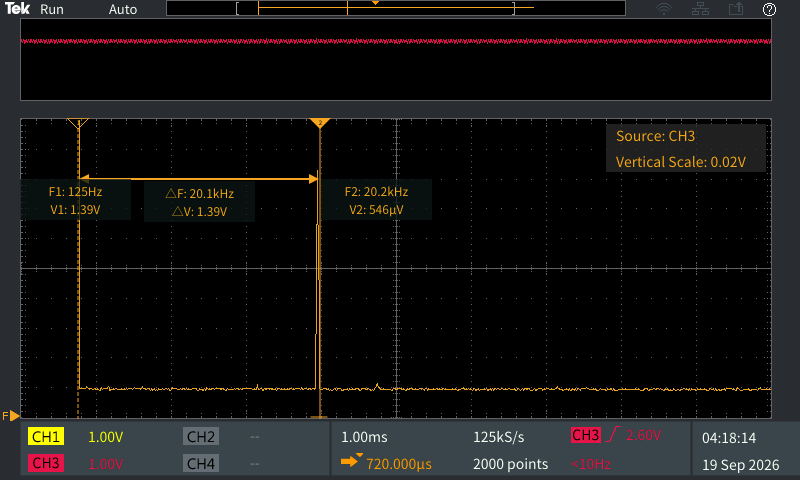
\includegraphics[width=0.48\textwidth]{exp_a3_tri_20kHz.png}}\\
\subfloat[20~kHz sine wave.]{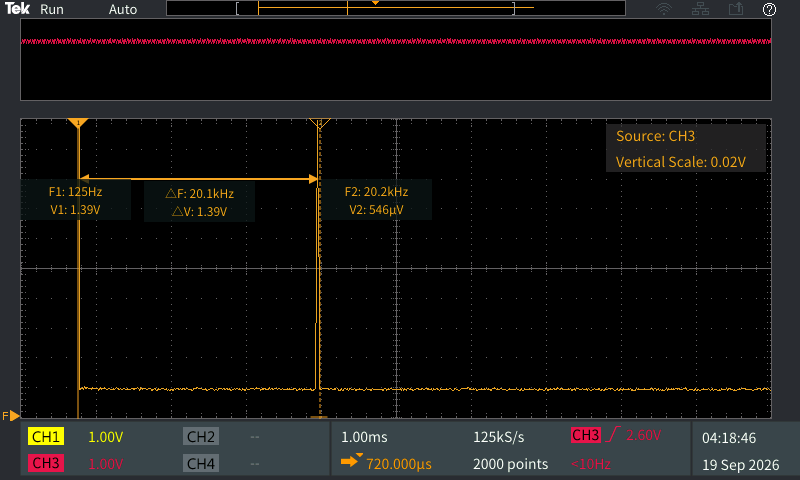
\includegraphics[width=0.48\textwidth]{exp_a3_sine_20kHz.png}}
\caption{Time-domain (top) and frequency-domain (bottom) oscilloscope
captures.}
\label{fig:exp_a3}
\end{figure}

%% ====================================================================
\section{Conclusion}
\label{sec:conc}

This lab has given the team a better understanding of not only the
instrumentation equipment and its calibration, but also of how simulation
software processes this information. Spending a lab tinkering with the
different oscilloscope functions has also contributed to a better overall
understanding of a critical piece of equipment, relevant not only to the
course but also to industry.

The biggest takeaways regarding the real-world versus simulation component of
the course, in the opinion of this group, concern the Fast Fourier Transform.
The team ran up against challenges during the lab with aliasing and with
configuring the equipment to view proper waveforms. Encountering the same
challenge again in the simulations allowed the group to target its weak points
and overcome them. Each member has internalized the Shannon--Nyquist sampling
theorem and has a greater understanding of its practical implications.

In simulation Activity~6, the triangle-wave harmonics were found to be very
similar to those found in the final experiment of the lab. The team can
therefore conclude that all systems are functional and, since the simulation
matched reality, that the simulation can be considered a good double check.

\end{document}
